\insertdesignoverview{The Black Hole Shooter}
{Shoot quickly and efficiently into the lander} % Goals of the mechanism
{Shooter_CAD.PNG}% CAD Image
{Shooter_Parts.JPG}% Build Image
{Elastic Sheet (25\% Spandex and 75\% Nylon), quarter inch MDF, lexan, one way bearing, steel ball, aluminum}% Materials ex. 0.25" MDF, Aluminum, etc
{Laser Cutting, 3D Printing, CNC Routing}% Manufacturing Processes ex. Laser Cut, 3D print, etc.

%\interesting{Our innovative glyph delivery mechanism, analyzed in depth}{Innovate:55}

\subsection*{How it Works}
 A ring is cut from MDF in an oval shape with a closely fitting larger ring. The larger ring is not continuous and aluminum material is screwed onto it to allow tightening. The elastic sheet is placed, taut, over the inner ring and under the larger ring. The larger ring is then tightened to secure the sheet. The steel ball is then placed in the center of the sheet and tied into the sheet on the underside. On the shaft of a REV core hex motor is a lever cut from lexan with a one way bearing secured within it. The lexan lever is then tied to the steel ball on the underside. The REV core hex motor rotates a 1.5 inch lexan lever down. When the lever rotates past 180 degrees, the one way bearing is allowed to freely move back to the original position. The lexan lever is tied to the elastic sheet and is pulled down up to 3 inches when it is rotated. 

\subsection*{Modelling \& Simulation}


\subsection*{Iteration}
The lever was initially made of quarter inch MDF which snapped due to the vertical force on the lever. The lever was also extended longer than it needed to be initially. The ring initially did not have a tightening ring around it, instead the sheet was tied to the ring.


\begin{figure}[htp]
\centering
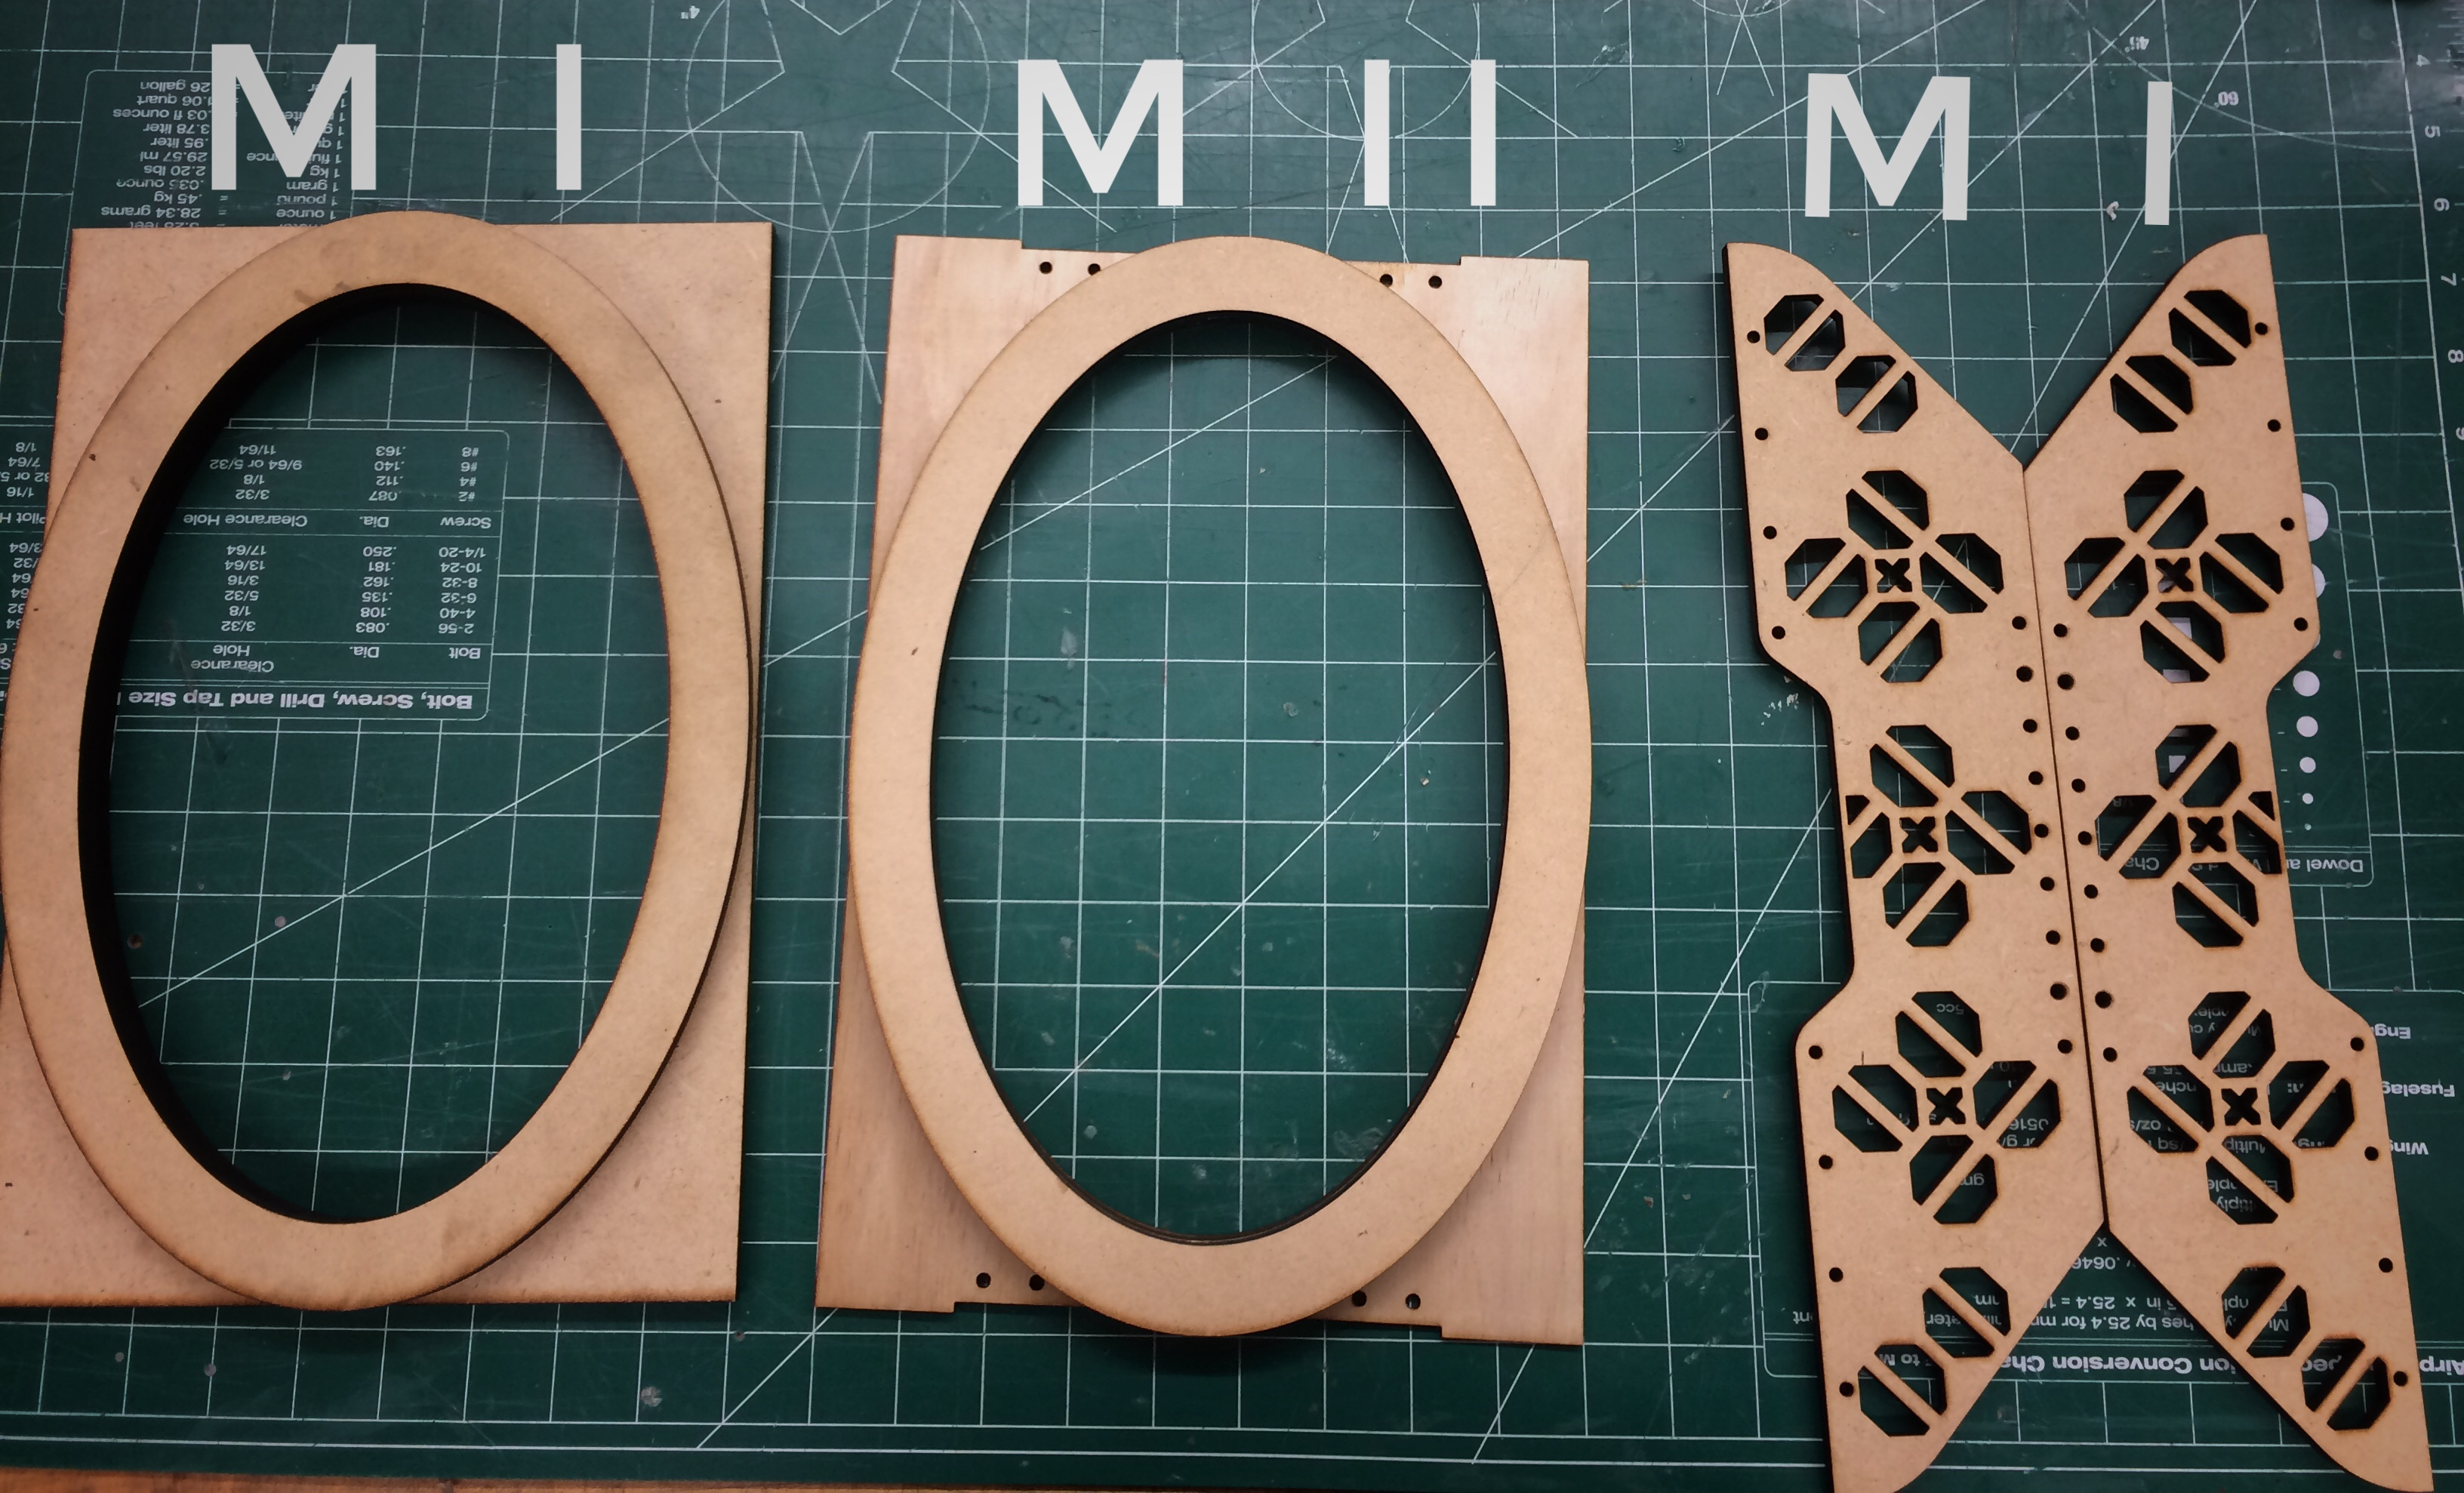
\includegraphics[width=.8\linewidth]{Design_Overview/Shooter_Iteration.JPG}
\caption{Design Iteration of the Shooter, Mark I and Mark II}
\label{fig:iteration}
\end{figure}

\begin{figure}[htp]
\centering
\begin{minipage}{.32\textwidth}
  \centering
  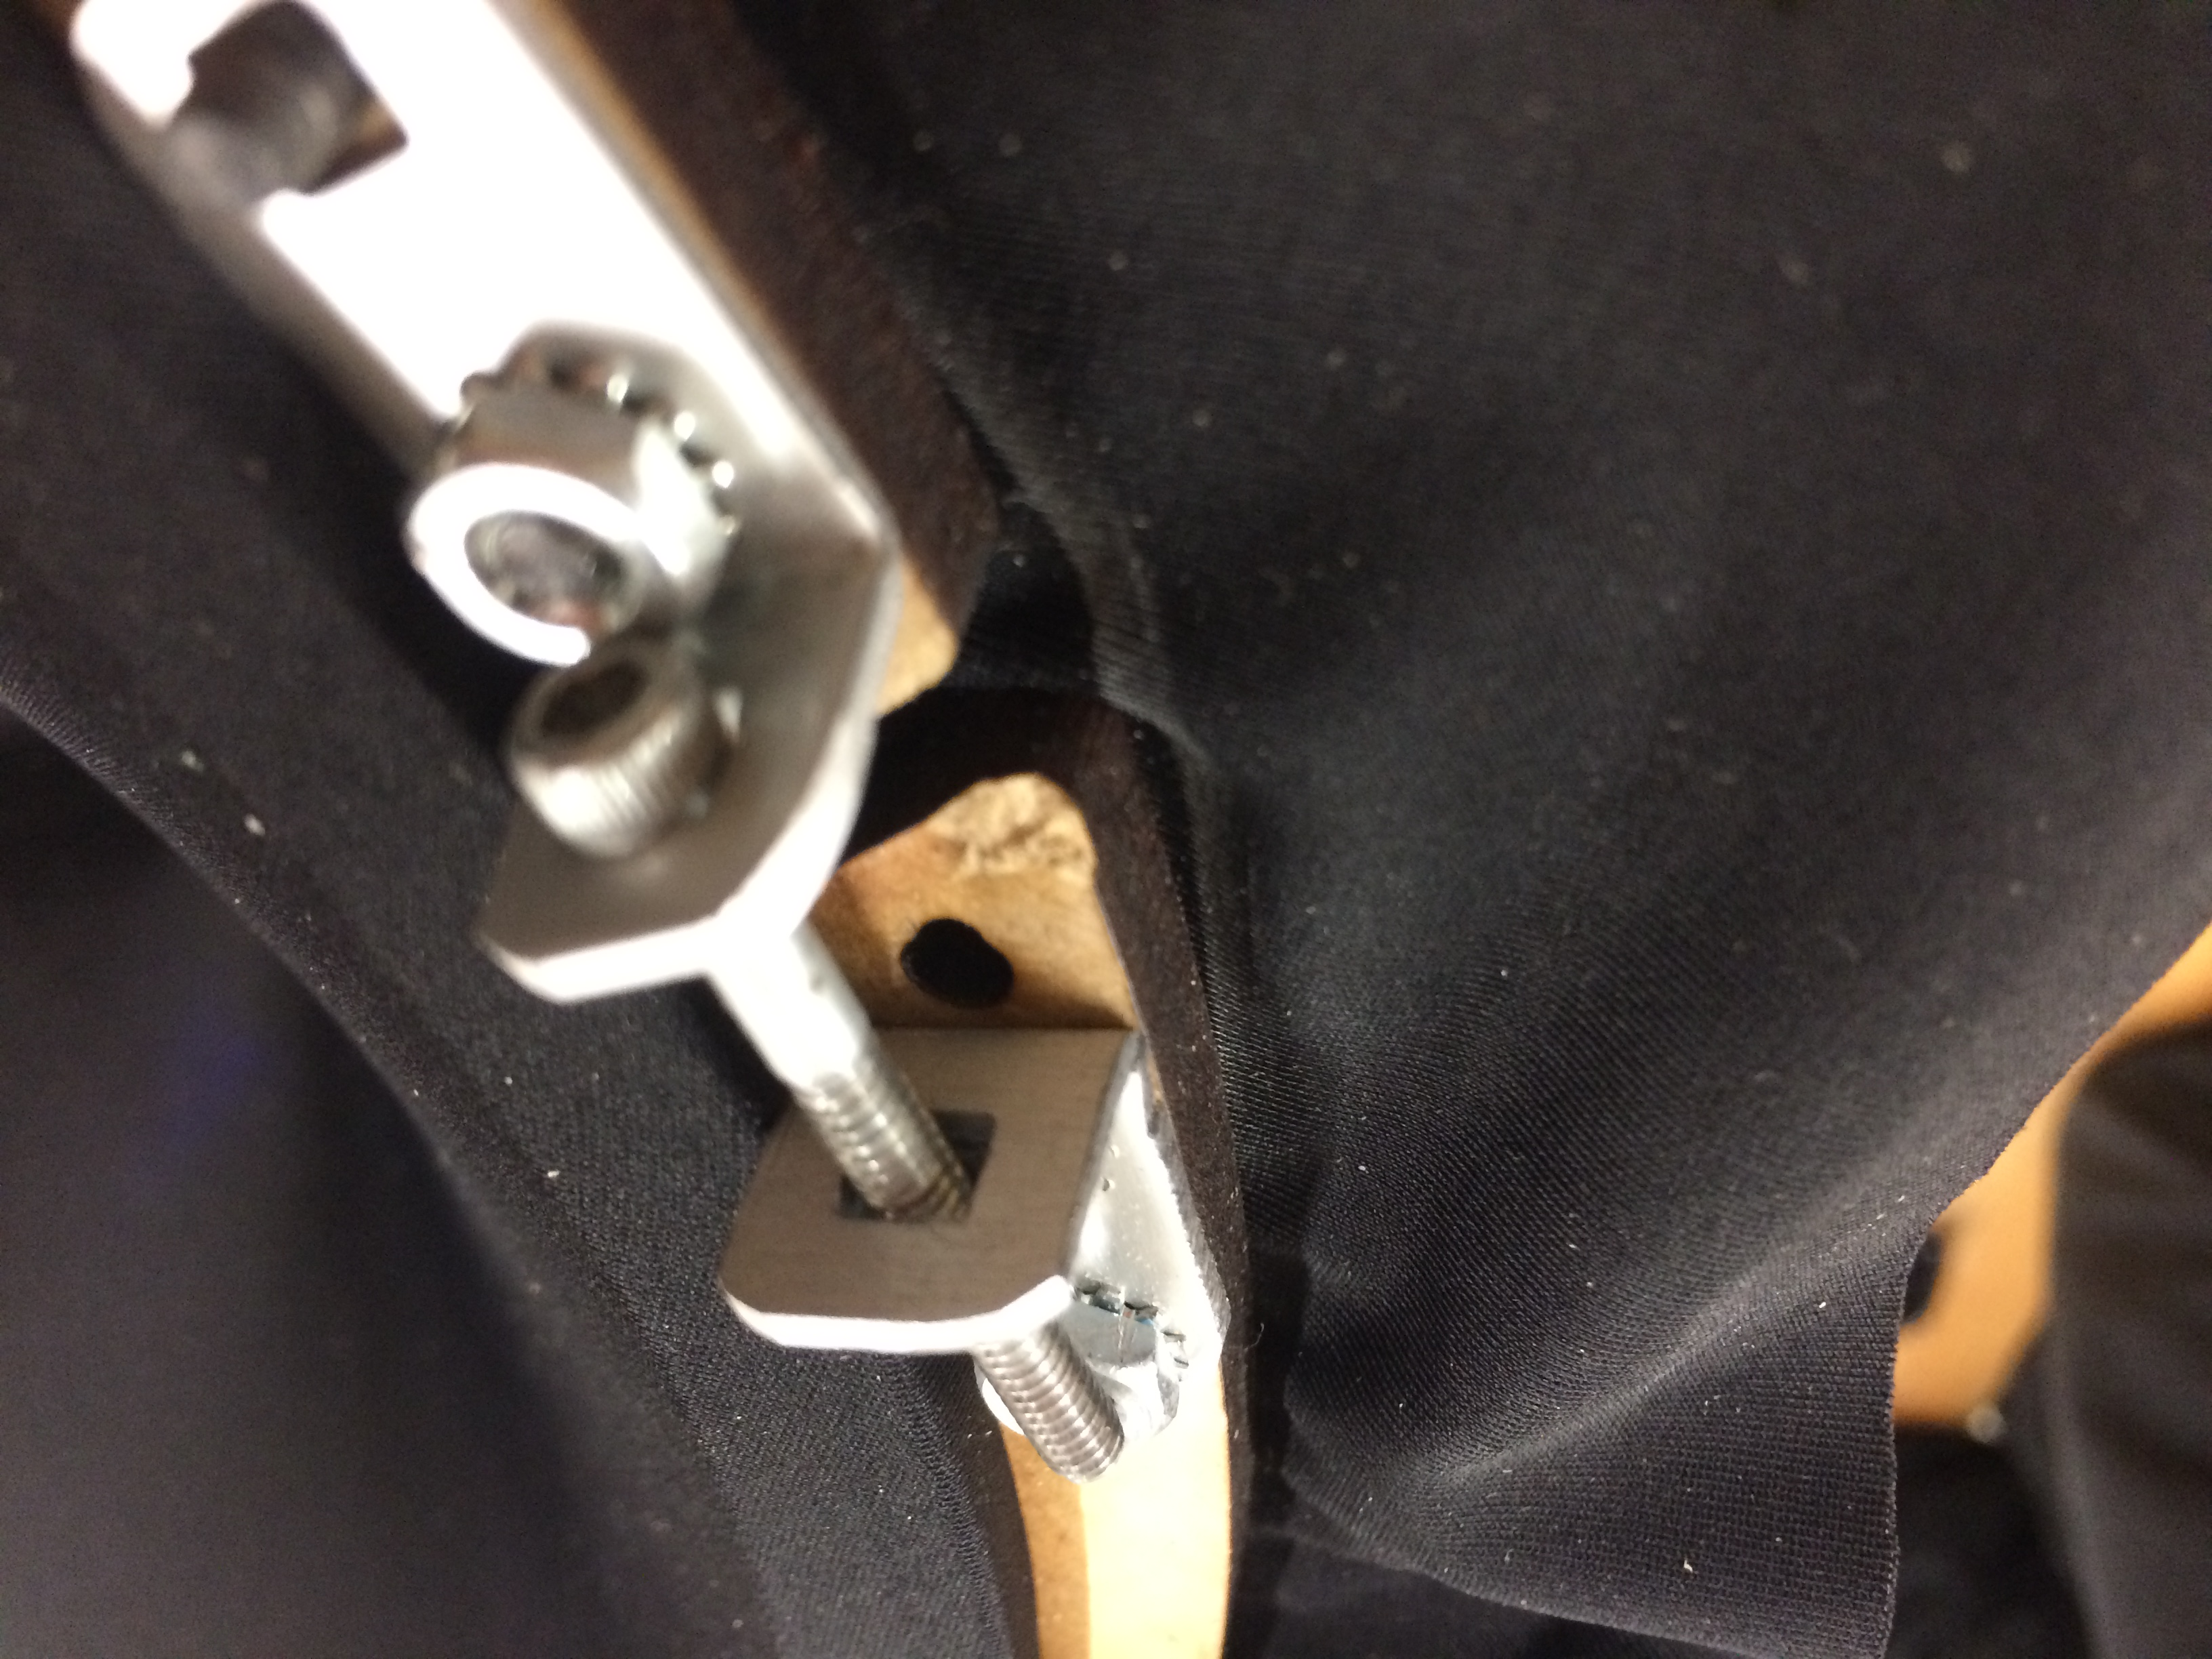
\includegraphics[width= .9\linewidth]{Design_Overview/Shooter_Left.JPG}
\end{minipage}%
\hfill
\begin{minipage}{.32\textwidth}
  \centering
  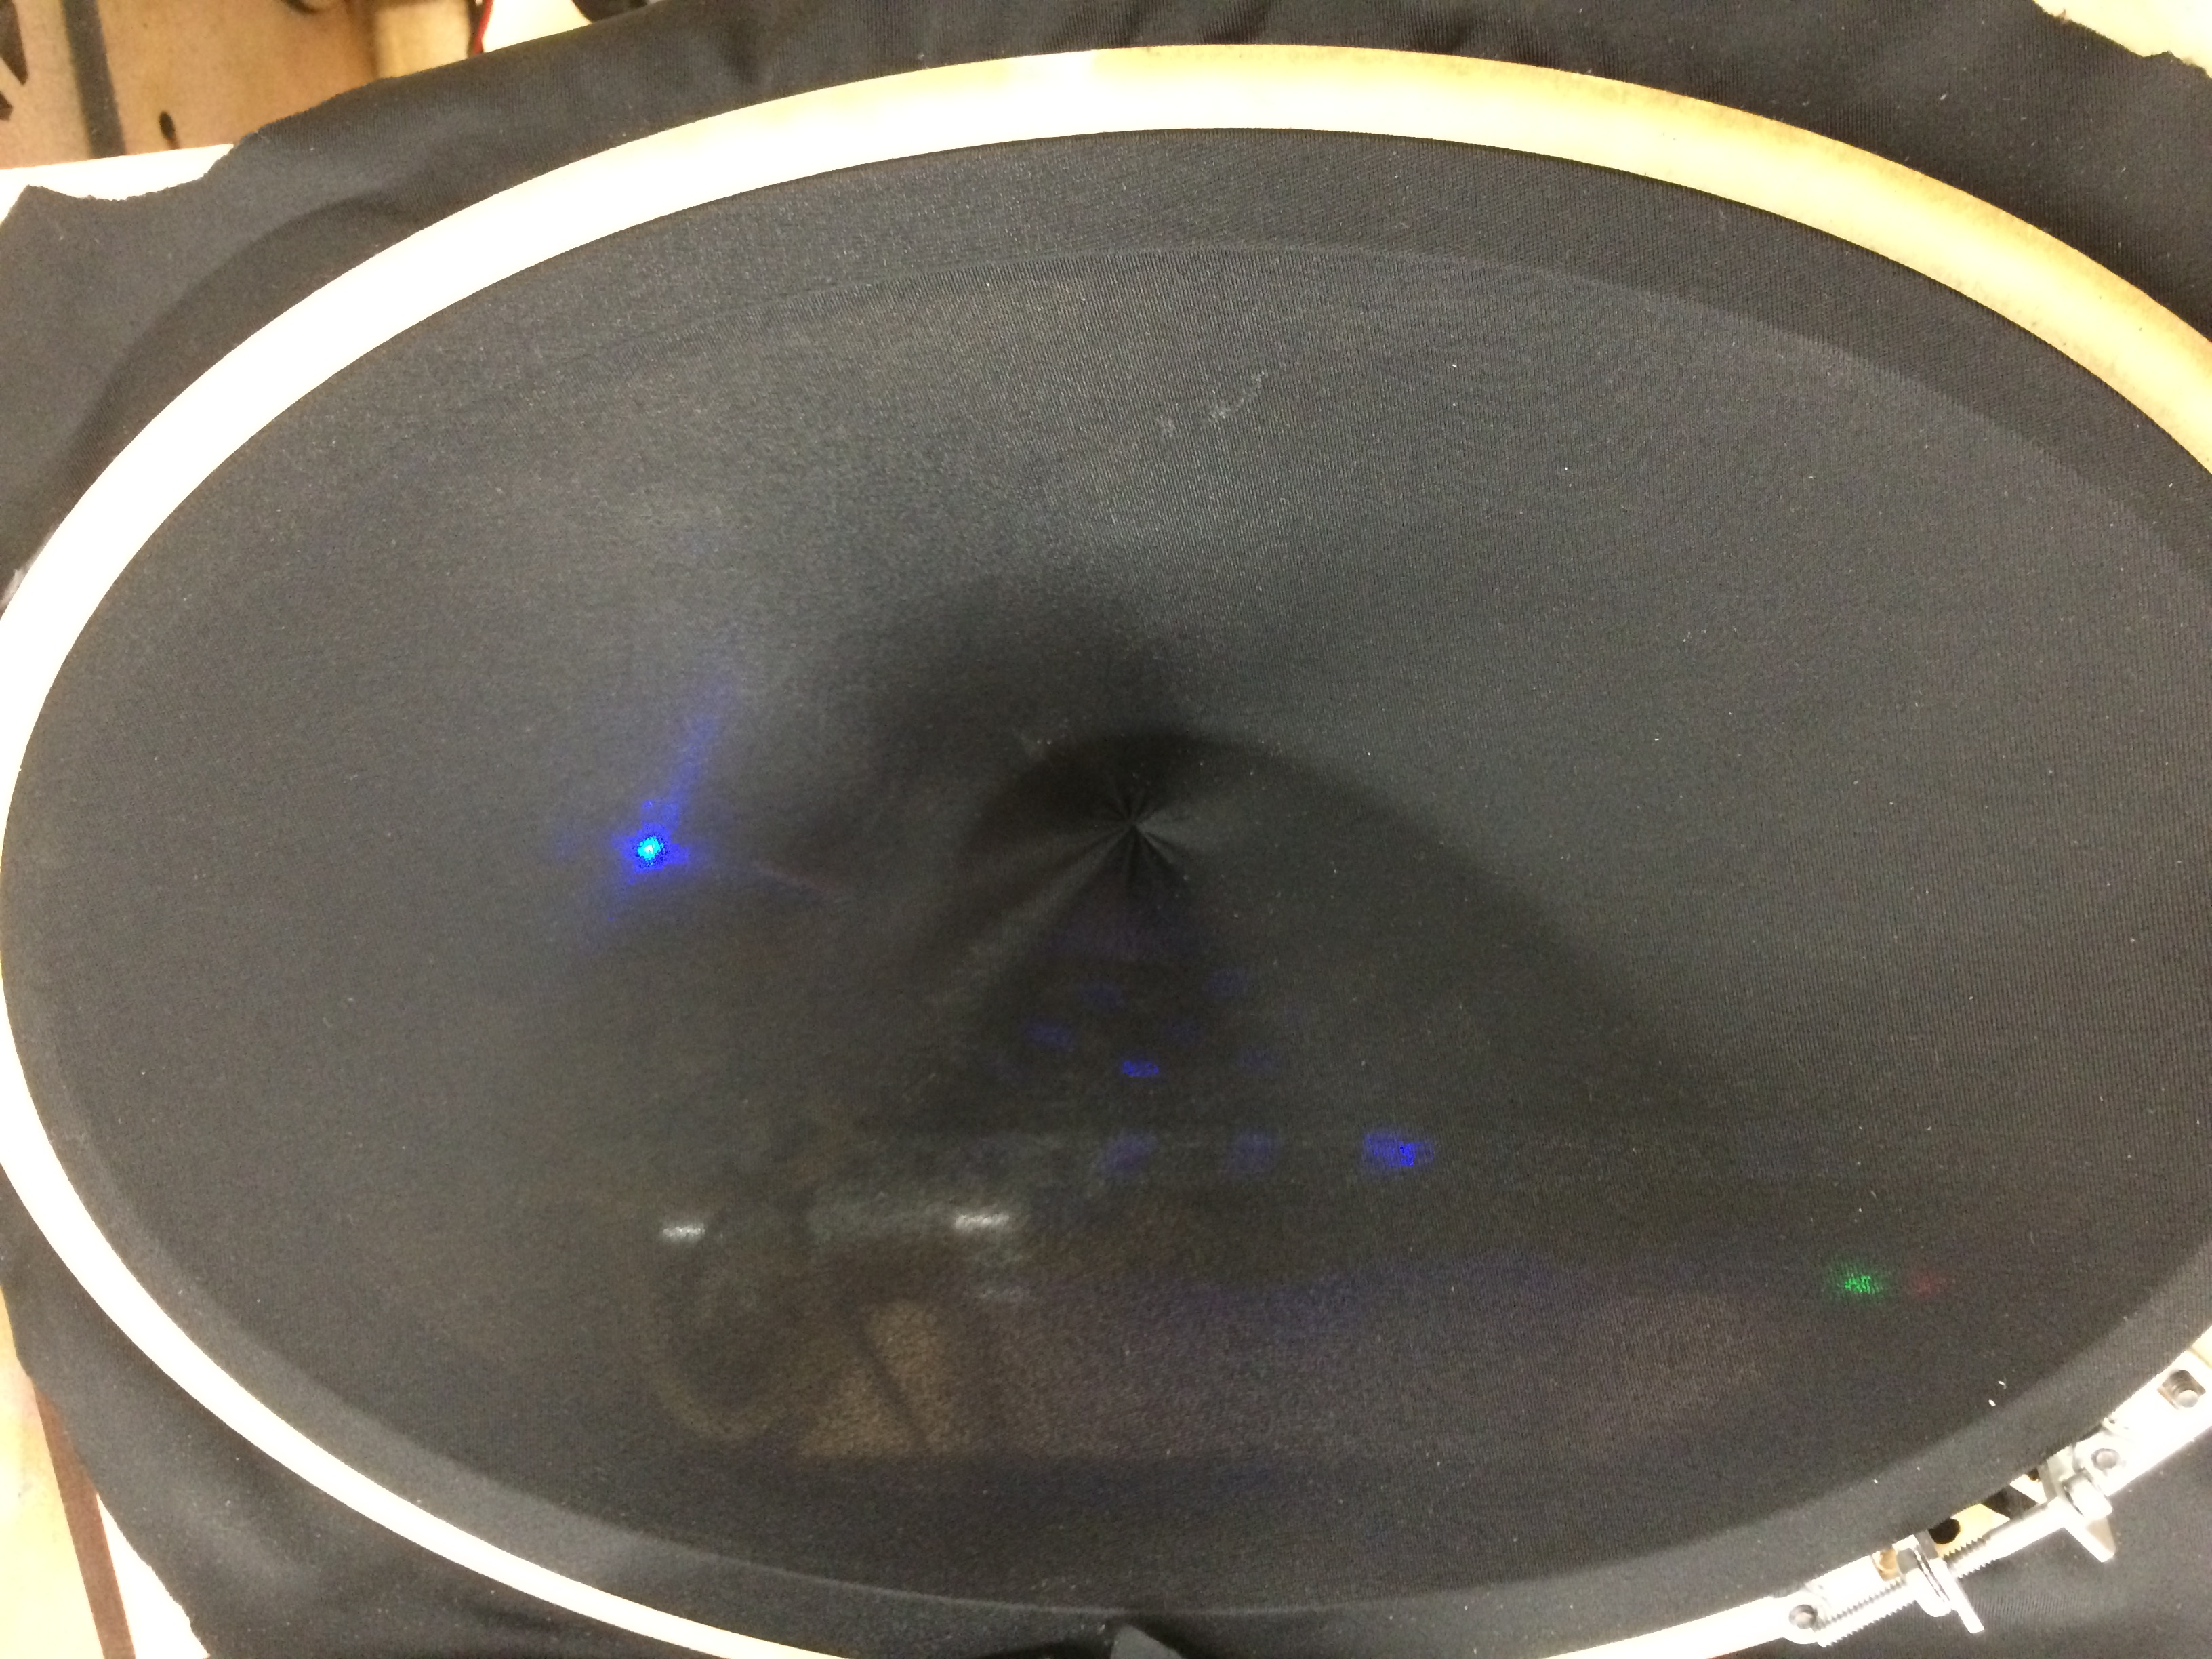
\includegraphics[width= .9\linewidth]{Design_Overview/Shooter_Front.JPG}
  \caption{Final Stabilization Arms, Mark III}
  \label{fig:Triple_Arm_IMG}
\end{minipage}%
  \hfill
\begin{minipage}{.32\textwidth}
  \centering
  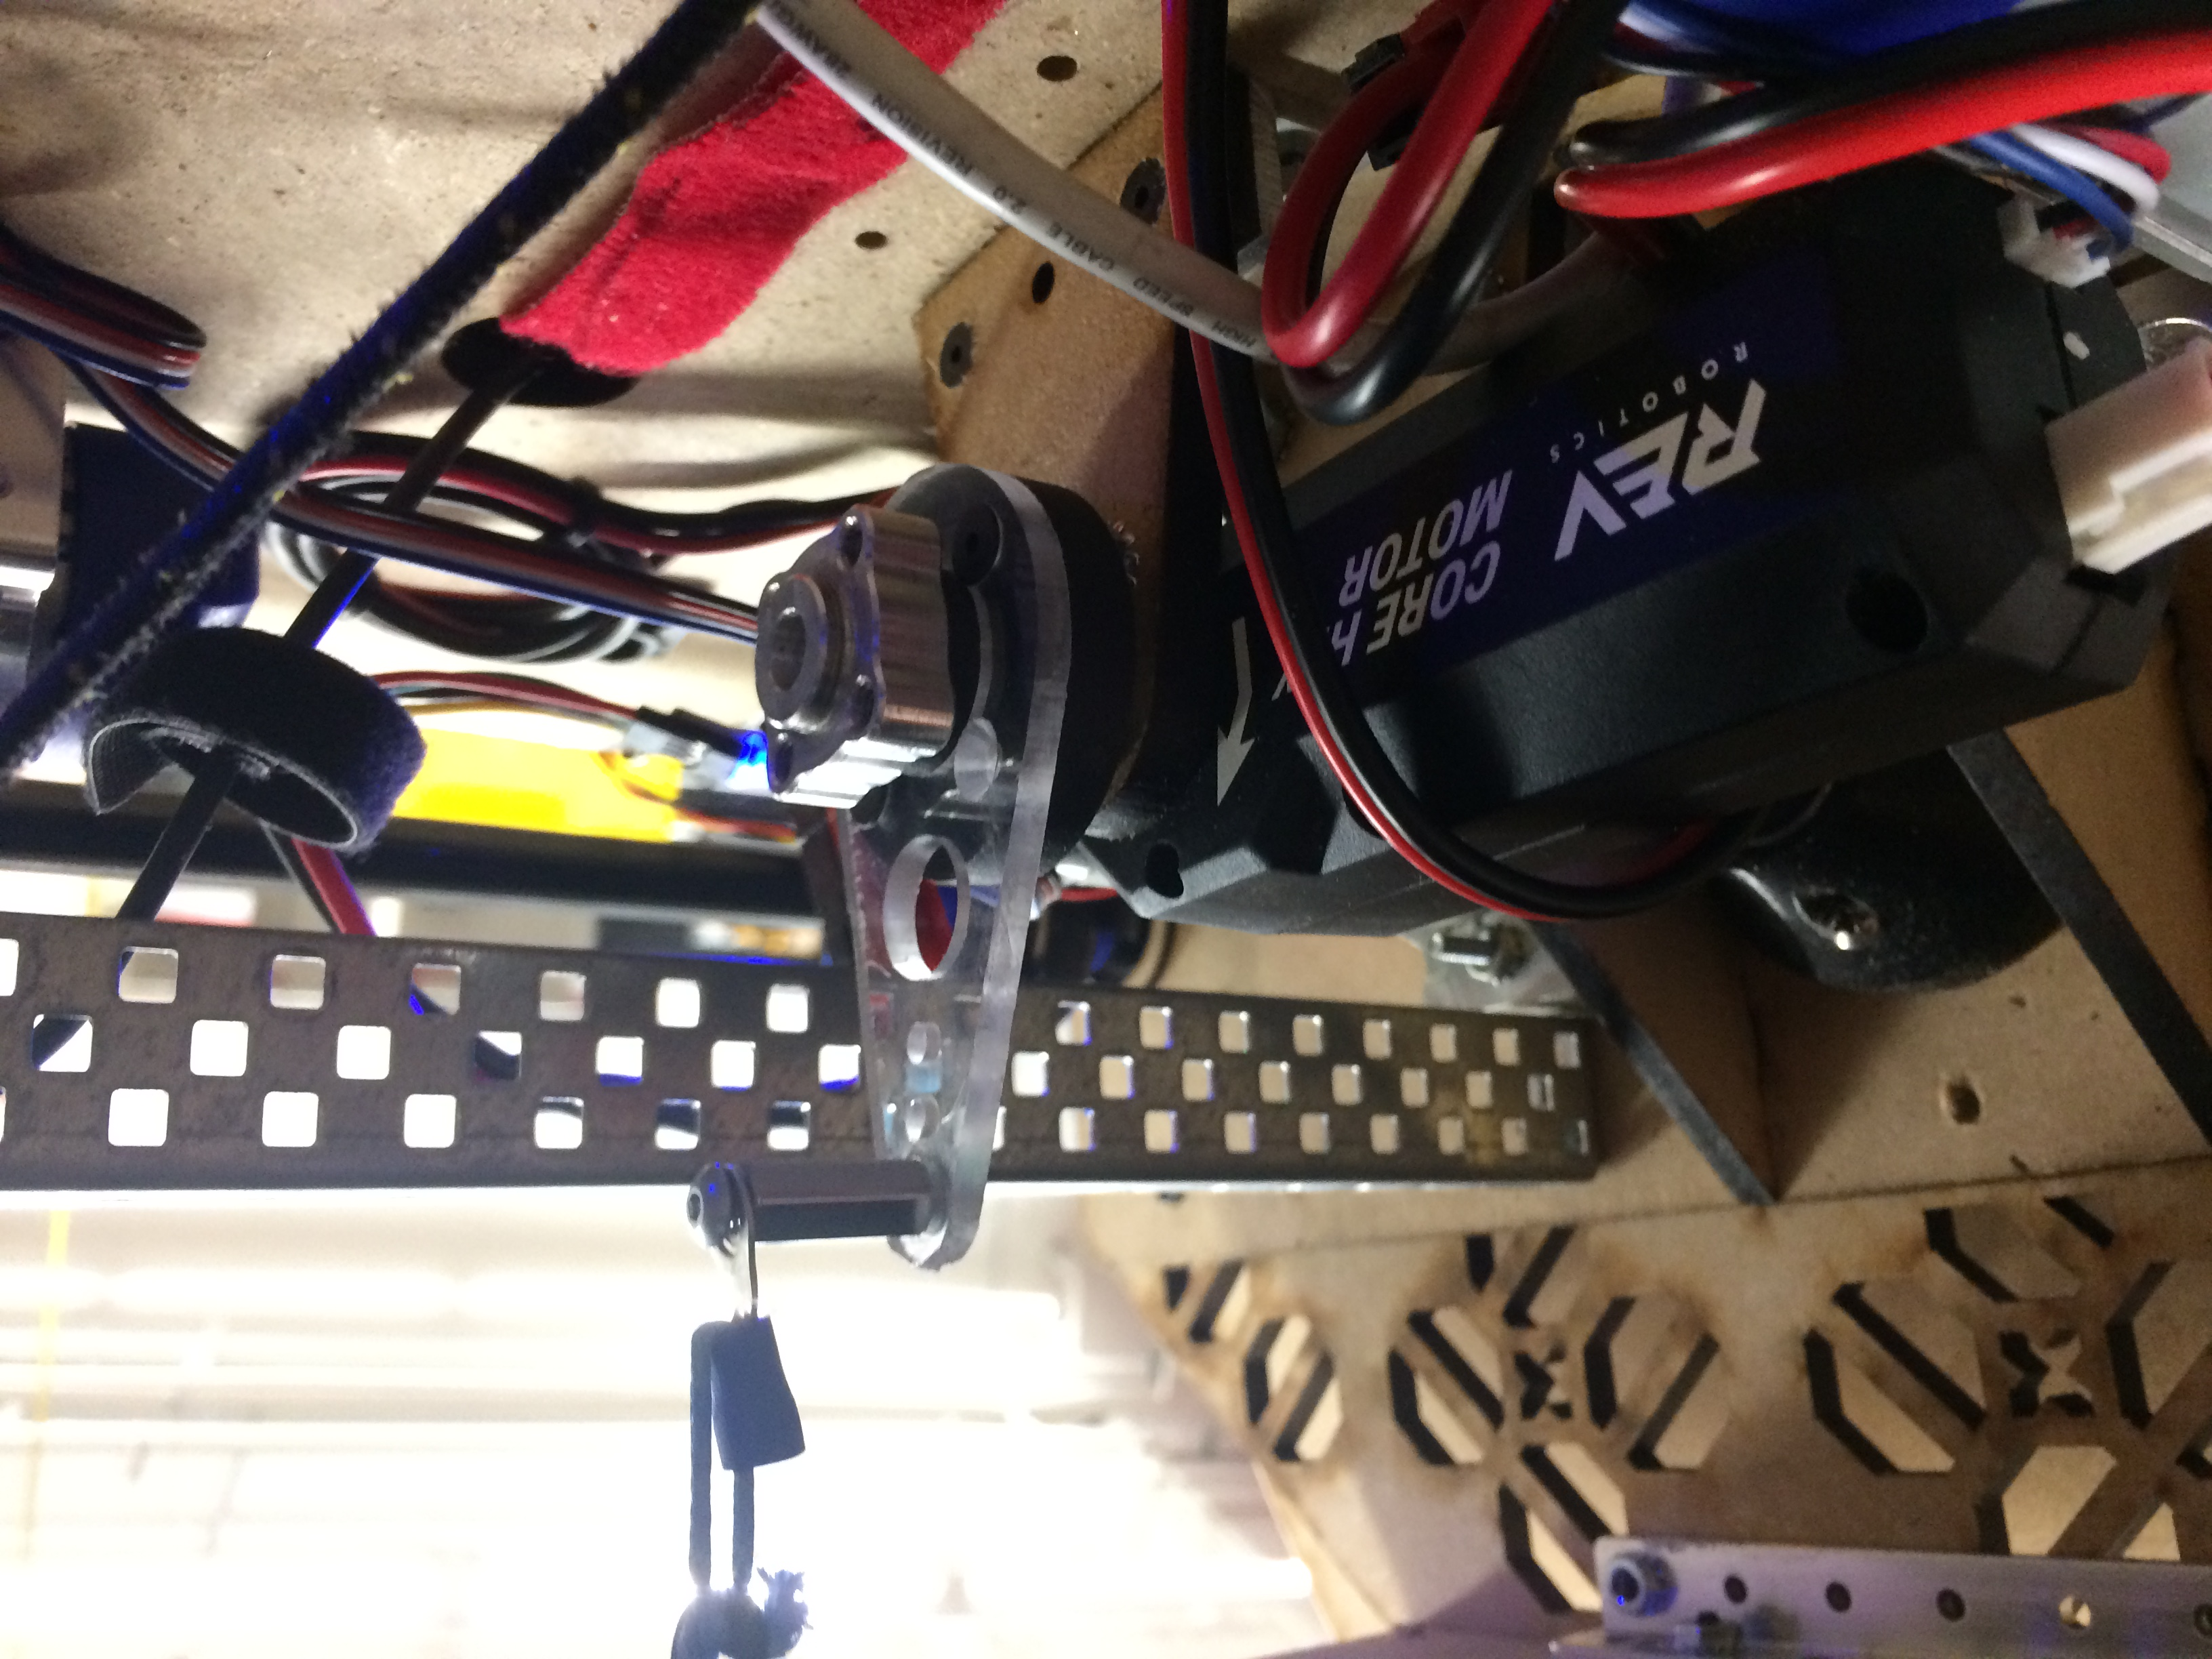
\includegraphics[width= .9\linewidth, angle=180]{Design_Overview/Shooter_Right.JPG}
\end{minipage}
\end{figure}

\subsection*{Sensors and Control}
An equation was made by the physics team to describe the peak vertical force on the system. Another equation was made to calculate the torque as the lever goes around. This is to ensure that the material and structure of the lever made will be able to support the tension from the sheet. Refer to the engineering section to find the formulas we calculated and used. 